\documentclass{beamer}

\usepackage{graphicx}
\usepackage{amsmath,amssymb,amsfonts}
\usepackage{tikz}
\usetikzlibrary{
  positioning,
  decorations.pathreplacing,
  shapes.misc,
  trees
}
\tikzset{file/.style={
  chamfered rectangle,
  chamfered rectangle corners=north west,
  draw, thick,
  fill=gray!30,
  anchor=west
}}
\tikzset{folder/.style={
  draw, thick,
  fill=brown!50,
  inner ysep=2mm,
  anchor=west
}}

\usetheme{Madrid}
\setbeamercovered{transparent=50}

\title[Baby XS]{Baby XS: Just enough to get you started\\YAPC::NA 2012}
\author{Joel Berger}
\institute[UIC]{University of Illinois at Chicago}
\date{June 15, 2012}

\usepackage{pygments}

\providecommand{\subitem}[1]{\begin{itemize}\item#1\end{itemize}}
\providecommand{\code}[1]{{\texttt{\scriptsize{#1}}}}

\begin{document}

\begin{frame}
  \maketitle
\end{frame}

\begin{frame}{What is XS?}
  \begin{itemize}
    \item XS the mechanism used to connect Perl and C
      \begin{itemize}
        \item write optimized functions
        \item access \code{C} libraries
      \end{itemize}
  \end{itemize}
  \vfill
  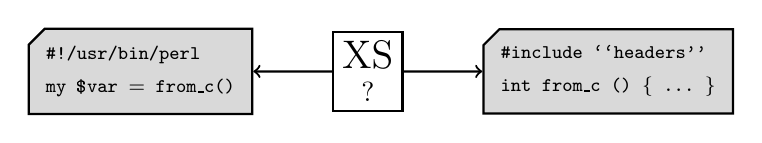
\begin{tikzpicture}
    \node (perl) [file,align=left] {\code{\#!/usr/bin/perl}\\\code{my \$var $=$ from\_c()}};
    \node (xs) [right=of perl,align=center,draw,thick] {\Large XS\\?};
    \node (c) [file,right=of xs,align=left] {\code{\#include ``headers''}\\\code{int from\_c () \{\ \ldots\ \}}};
    \draw [thick,<-] (perl) -- (xs);
    \draw [thick,->] (xs) -- (c);
  \end{tikzpicture}
  \vfill
  \begin{itemize}
    \item XS is C functions/macros provided by Perl headers
    \item XS is also XS-preprocessesor directives
  \end{itemize}
\end{frame}

\begin{frame}{What are ``baby'' languages?}
  \begin{block}{``Baby'' Langauge}
    The naive code that new programmers write,\\a simple subset of the full language
  \end{block}
  \begin{itemize}
    \item ``Baby Perl''
      \begin{itemize}
        \item no \code{map} / \code{grep}
        \item no references
        \item avoids \code{\$\_}
      \end{itemize}
    \item ``Full XS'' is powerful but is lots to learn
    \item ``Baby XS'' 
     \begin{itemize}
       \item looks like C
       \item behaves like Perl
     \end{itemize}
  \end{itemize}
\end{frame}

\begin{frame}{Baby XS}
  \begin{block}{What is Baby XS?}
    Some ``easy'' idioms and rules-of-thumb to keep XS from becoming overwhelming
  \end{block}
  \begin{itemize}
    \item<2-> ignores typemaps
    \item<3-> uses Perl datatype-specific functions from \code{perldoc perlguts}
    \item<4-> ignores most of the XSpp commands
    \item<5-> ignores stack macros
    \item<6-> avoids (most) issues of ``mortalization''
    \item<7-> uses a Perl-level function wrapper to munge input/output if needed
    \item<8-> expands to ``real'' XS
  \end{itemize}
\end{frame}

\begin{frame}{Types}
  XS has types that are like their Perl counterparts
  \begin{itemize}
    \item Scalar $\Leftrightarrow$ \code{SV*}
    \item Array $\Leftrightarrow$ \code{AV*}
    \item Hash $\Leftrightarrow$ \code{HV*}
  \end{itemize}
  \uncover<2->{
    Of course XS is really C so it also has types like
    \begin{itemize}
      \item \code{int}
      \item \code{double}
      \item \code{char*}
    \end{itemize}
    \ldots which Perl converts to/from \code{SV*} when used as arguments or return value
  }
  \begin{block}<3->{For Future Reference}
    You can add you own automatic conversions via a \code{Typemap} file
  \end{block}
\end{frame}

\begin{frame}[fragile]{Sample XS File}
  \scriptsize
  \begin{columns}
    \begin{column}{0.54\linewidth}
      \begin{block}{}
        \begin{Verbatim}[commandchars=\\\{\}]
\PY{c+cp}{\PYZsh{}}\PY{c+cp}{include "EXTERN.h"}
\PY{c+cp}{\PYZsh{}}\PY{c+cp}{include "perl.h"}
\PY{c+cp}{\PYZsh{}}\PY{c+cp}{include "XSUB.h"}

\PY{k+kt}{int} \PY{n+nf}{meaning} \PY{p}{(}\PY{p}{)} \PY{p}{\PYZob{}} \PY{k}{return} \PY{l+m+mi}{42} \PY{p}{\PYZcb{}}
\PY{k+kt}{void} \PY{n+nf}{greet} \PY{p}{(}\PY{k+kt}{char}\PY{o}{*} \PY{n}{name}\PY{p}{)} 
\PY{p}{\PYZob{}}
  \PY{n}{printf}\PY{p}{(} \PY{l+s}{"}\PY{l+s}{Hello \PYZpc{}s}\PY{l+s+se}{\PYZbs{}n}\PY{l+s}{"}\PY{p}{,} \PY{n}{name} \PY{p}{)} 
\PY{p}{\PYZcb{}}

\PY{n}{MODULE} \PY{o}{=} \PY{n}{My}\PY{o}{:}\PY{o}{:}\PY{n}{Module}    \PY{n}{PACKAGE} \PY{o}{=} \PY{n}{My}\PY{o}{:}\PY{o}{:}\PY{n}{Module}

\PY{k+kt}{int}
\PY{n}{meaning} \PY{p}{(}\PY{p}{)}

\PY{k+kt}{void}
\PY{n}{greet} \PY{p}{(}\PY{n}{name}\PY{p}{)}
    \PY{k+kt}{char}\PY{o}{*} \PY{n}{name}
\end{Verbatim}

      \end{block}
    \end{column}
    \begin{column}{0.44\linewidth}
      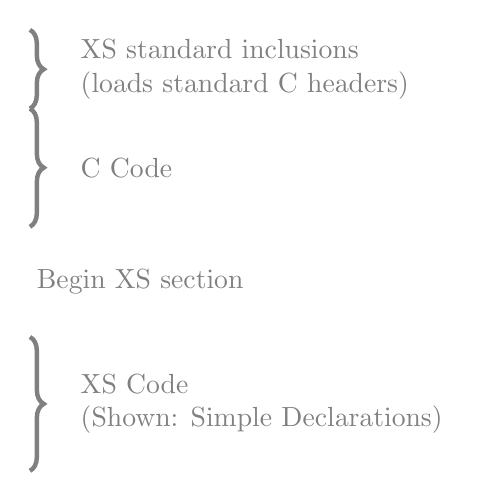
\begin{tikzpicture}
        \visible<2->{
          \draw
            [decoration={brace,amplitude=0.5em},decorate,ultra thick,gray]
            (0,2.7) --
            (0,1.7)
              node [right=5mm,pos=0.5,align=left] {XS standard inclusions\\(loads standard C headers)}
          ;
        }
        \visible<3->{
          \draw
            [decoration={brace,amplitude=0.5em},decorate,ultra thick,gray]
            (0,1.7) --
            (0,0.2)
              node [right=5mm,pos=0.5] {C Code}
          ;
        }
        \visible<4->{
          \node at (1.4,-0.5) [gray] {Begin XS section};
        }
        \visible<5->{
          \draw
            [decoration={brace,amplitude=0.5em},decorate,ultra thick,gray]
            (0,-1.2) --
            (0,-2.9)
              node [right=5mm,pos=0.5,align=left] {XS Code\\(Shown: Simple Declarations)}
          ;
        }
      \end{tikzpicture}
    \end{column}
  \end{columns}
\end{frame}

\begin{frame}{Using \texttt{SV*}s}
  SV* behave like scalars in Perl, but have different actions based on type
  \begin{columns}
    \begin{column}{0.49\linewidth}
      \begin{block}{Creating}
        \begin{itemize}
          \item \code{SV* newSViv(IV)}
          \item \code{SV* newSVnv(double)}
          \item \code{SV* newSVpvf(const char*, ...)}
          \item \code{SV* newSVsv(SV*)}
        \end{itemize}
      \end{block}
    \end{column}
    \begin{column}{0.49\linewidth}
      \begin{block}{Accessing}<2->
        \begin{itemize}
          \item \code{int SvIV(SV*)}
          \item \code{double SvNV(SV*)}
          \item \code{char* SvPV(SV*, STRLEN len)}
          \item \code{char* SvPV\_nolen(SV*)}
        \end{itemize}
      \end{block}
    \end{column}
  \end{columns}
  \begin{block}{Other Actions}<3->
    Plenty of other Perl-like actions, see \code{perldoc perlguts} for more.
    \begin{itemize}
      \item \code{SvTRUE(SV*)} --- test for ``truth''
      \item \code{sv\_catsv(SV*, SV*)} --- join strings
    \end{itemize}
  \end{block}
\end{frame}

\begin{frame}[fragile]{Using \texttt{AV*}s and \texttt{HV*}s}
  \begin{itemize}
    \item Perl-like functions, e.g. \code{av\_push}
    \item filled with \code{SV*} objects
    \item used as argument or return value, Perl uses references
    \item ``mortalization'' problem for returns
    \item recommended Baby XS way to return multiple values:
  \end{itemize}
  \vfill
  \begin{block}{}
    \scriptsize
    \begin{Verbatim}[commandchars=\\\{\}]
\PY{n}{AV}\PY{o}{*} \PY{n+nf}{foo} \PY{p}{(}\PY{p}{)} \PY{p}{\PYZob{}}
  \PY{n}{AV}\PY{o}{*} \PY{n}{ret} \PY{o}{=} \PY{n}{newAV}\PY{p}{(}\PY{p}{)}\PY{p}{;}
  \PY{c+cm}{/* fix mortalization */}
  \PY{n}{sv\PYZus{}2mortal}\PY{p}{(}\PY{p}{(}\PY{n}{SV}\PY{o}{*}\PY{p}{)}\PY{n}{ret}\PY{p}{)}\PY{p}{;}

  \PY{n}{av\PYZus{}push}\PY{p}{(}\PY{n}{ret}\PY{p}{,} \PY{n}{newSViv}\PY{p}{(}\PY{l+m+mi}{1}\PY{p}{)}\PY{p}{)}\PY{p}{;}
  \PY{n}{av\PYZus{}push}\PY{p}{(}\PY{n}{ret}\PY{p}{,} \PY{n}{newSVpvf}\PY{p}{(}\PY{l+s}{"}\PY{l+s}{\PYZpc{}s}\PY{l+s}{"}\PY{p}{,} \PY{l+s}{"}\PY{l+s}{bar}\PY{l+s}{"}\PY{p}{)}\PY{p}{)}\PY{p}{;}

  \PY{c+cm}{/* return [ 1, "bar" ] */}
  \PY{k}{return} \PY{n}{ret}\PY{p}{;}
\PY{p}{\PYZcb{}}
\end{Verbatim}

  \end{block}
\end{frame}

\begin{frame}[fragile]{Sample Perl Module}
  \begin{block}{}
    \scriptsize
    \begin{Verbatim}[commandchars=\\\{\}]
\PY{n+nb}{package} \PY{n}{MyModule}\PY{p}{;}

\PY{k}{use} \PY{n}{strict}\PY{p}{;} \PY{k}{use} \PY{n}{warnings}\PY{p}{;}
\PY{k}{our} \PY{n+nv}{\PYZdl{}}\PY{n+nv}{VERSION} \PY{o}{=} \PY{l+s}{'0.01'}\PY{p}{;}

\PY{n+nb}{require} \PY{n}{XSLoader}\PY{p}{;}
\PY{n+nn}{XSLoader::}\PY{n}{load}\PY{p}{(}\PY{p}{)}\PY{p}{;}

\PY{k}{sub }\PY{n+nf}{myfunc} \PY{p}{\PYZob{}}
  \PY{k}{my} \PY{n+nv}{@}\PY{n+nv}{args} \PY{o}{=} \PY{n+nv}{@}\PY{n+nv}{\PYZus{}}\PY{p}{;}
  \PY{k}{my} \PY{n+nv}{\PYZdl{}}\PY{n+nv}{ret} \PY{o}{=} \PY{n}{c\PYZus{}func}\PY{p}{(}\PY{n+nv}{@}\PY{n+nv}{args}\PY{p}{)}\PY{p}{;}
  \PY{k}{return} \PY{n+nb}{wantarray} \PY{p}{?} \PY{n+nv}{@\PYZdl{}}\PY{n+nv}{ret} \PY{p}{:} \PY{n+nv}{\PYZdl{}}\PY{n+nv}{ret}\PY{o}{-}\PY{o}{>}\PY{p}{[}\PY{l+m+mi}{0}\PY{p}{]}\PY{p}{;}
\PY{p}{\PYZcb{}}
\end{Verbatim}

  \end{block}
  \begin{itemize}
    \item Wrap C function calls in Perl subs
    \begin{itemize}
      \item munge inputs / outputs easier
      \item abstraction if C function changes
    \end{itemize}
    \item Export the Perl function (if desired)
  \end{itemize}
\end{frame}

\begin{frame}{Building/Packaging (Module::Build)}
  \begin{columns}
    \begin{column}{0.49\linewidth}
      \begin{block}{Structure}
        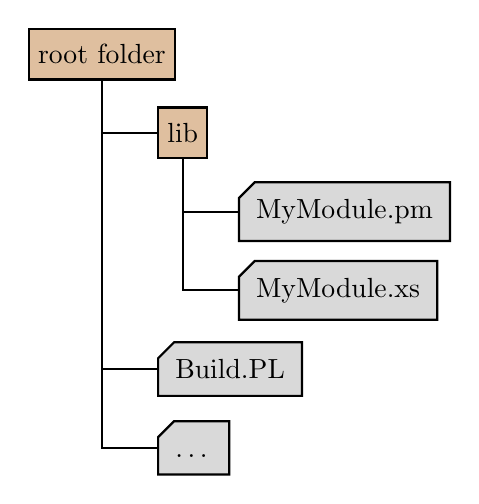
\begin{tikzpicture}
          [
            grow via three points={
              one child at    (0.7,-1) and
              two children at (0.7,-1) and (0.7,-2)
            },
            edge from parent path={[thick] (\tikzparentnode.south) |- (\tikzchildnode.west)}
          ]
          \node [folder] {root folder}
            child { node [folder] {lib}
              child { node [file] {MyModule.pm} }
              child { node [file] {MyModule.xs} }
            }
            child [missing] {}
            child [missing] {}
            child { node [file] {Build.PL} }
            child { node [file] { \ldots \vphantom{X}} }
          ;
        \end{tikzpicture}
      \end{block}
      \vspace{4mm}
    \end{column}
    \begin{column}{0.49\linewidth}
      \scriptsize
      \begin{block}{Build.PL}
        \begin{Verbatim}[commandchars=\\\{\}]
\PY{k}{use} \PY{n}{strict}\PY{p}{;}
\PY{k}{use} \PY{n}{warnings}\PY{p}{;}

\PY{k}{use} \PY{n+nn}{Module::Build}\PY{p}{;}

\PY{k}{my} \PY{n+nv}{\PYZdl{}}\PY{n+nv}{builder} \PY{o}{=} \PY{n+nn}{Module::Build}\PY{o}{-}\PY{o}{>}\PY{k}{new}\PY{p}{(}
    \PY{n}{module\PYZus{}name}       \PY{o}{=}\PY{o}{>} \PY{l+s}{'MyModule'}\PY{p}{,}
    \PY{n}{dist\PYZus{}author}       \PY{o}{=}\PY{o}{>} \PY{l+s}{'Joel Berger'}\PY{p}{,}
    \PY{n}{license}           \PY{o}{=}\PY{o}{>} \PY{l+s}{'perl'}\PY{p}{,}
    \PY{n}{configure\PYZus{}requires} \PY{o}{=}\PY{o}{>} \PY{p}{\PYZob{}}
      \PY{l+s}{'Module::Build'} \PY{o}{=}\PY{o}{>} \PY{l+m+mf}{0.38}\PY{p}{,}
    \PY{p}{\PYZcb{}}\PY{p}{,}
    \PY{n}{build\PYZus{}requires}    \PY{o}{=}\PY{o}{>} \PY{p}{\PYZob{}}
      \PY{l+s}{'ExtUtils::CBuilder'} \PY{o}{=}\PY{o}{>} \PY{l+m+mi}{0}\PY{p}{,}
    \PY{p}{\PYZcb{}}\PY{p}{,}    
    \PY{n}{extra\PYZus{}linker\PYZus{}flags} \PY{o}{=}\PY{o}{>} \PY{l+s}{'-lsomelib'}\PY{p}{,}
\PY{p}{)}\PY{p}{;}

\PY{n+nv}{\PYZdl{}}\PY{n+nv}{builder}\PY{o}{-}\PY{o}{>}\PY{n}{create\PYZus{}build\PYZus{}script}\PY{p}{;}
\end{Verbatim}

      \end{block}
    \end{column}
  \end{columns}
\end{frame}

\begin{frame}{Other C Connections}
  There are other mechanisms for hooking into C
  \begin{itemize}
    \item \code{Inline::C}
      \begin{itemize}
        \item write C in your Perl script
        \item builds/loads the XS for you!
        \item great for quick checks
      \end{itemize}
    \item \code{PDL::PP}
      \begin{itemize}
        \item part of \code{PDL}
        \item special C interaction for fast numerical processing
        \item has its own syntax
      \end{itemize}
  \end{itemize}
\end{frame}

\begin{frame}{Acknowledgements}
  
\includegraphics[width=0.7\linewidth]{uic}
  \begin{itemize}
    \item Graduate College Dean's Fellowship (Major Funding)
    \item LAS Ph.D. Travel Award (Conference Funding)
  \end{itemize}
\end{frame}

\end{document}
